\chapter{图论 - 图的表示, 种类}
\begin{figure}[ht]
  \centering
  
\includegraphics[width=1\textwidth]{asset/茶桁的AI秘籍_Math_24.png}
\end{figure}

\newpage

Hi,你好. 我是茶桁. 

之前的一节课中,我们了解了图的来由和构成,简单的理解了一下图的一些相关概念. 那么这节课,我们要了解一下图的表示,种类. 相应的,我们中间需要穿插一些新的知识点用于更好的去理解图,比如说邻接矩阵. 

\section{图的表示}

我们一般用什么样的形式来表示图呢? 方法其实也是非常多样的. 一开始说到定义的时候,就采用的集合表示的方法. 集合表示什么意思呢? 就是我们定义里面所说的那样,$G = <V, E>$,一个序偶. 

V和E, 集合里面的元素各是多少, 用集合的那种表达式可以展开就行了, 这个就叫做「集合表示」. 

图形表示也很常见, 上节课一开始说到这个图的由来,包括我一直跟大家说这个图是一个怎样的东西的时候,都是采用的这种非常形象直观的方式去给大家进行讲解. 

那它有什么样的特征呢? 图里面V中结点,都是用小圆圈来表示的,这个有序的结点对$<u,v>$表示由结点u指向结点v的有向边e. 这个时候如果它是有方向的,那我们就把这条边的u称为e的始点,因为它是由u指向v的,v称为e的终点,或者把它俩统称为端点. 

如果是一个无向图,首先我们需要先来理解一下有向、无向是一个什么样的意思. 比如,在一个图里面,
我们在里边是没有箭头的,它就是一个无向图. 如果是由v3指向v2,那在就有一个箭头了,它就是一个有向图,或者说有向边. 

大家注意,对于无序的情况的,表示符号是用圆括号来表示的,和上面的那种尖括号是不一样的,这个要区别一下. 那无序的结点对$(u,v)$或者$(v,u)$,表示结点u和结点v之间的无向边. 这里就不区分始点终点了,统称为端点,此时仅称u, v为边e的两个端点. 如果把v放前面,u放后面也是一样,等价. 因为它是无序的. 

我们来看一下,怎么样根据这个图的几何表示给它转换成图形表示. 首先告诉你这个图是一个集合表现的形式,是由v和e表示的. 

设图$G=<V, E>$, 且$V = \{v_1,v_2,v_3,v_4,v_5\}$, $E = \{e_1,e_2,e_3,e_4,e_5,e_6\}$

我们只知道顶点和边还不够,还要知道这些边是连接着哪两个顶点的. 

图中的边为:  
\begin{align*}
  e_1=(v_1,v_2), \quad e_2=<v_1,v_3>, \quad e_3=(v_1,v_4), \\ 
  e_4=(v_2,v_3), \quad e_5=<v_3,v_2>, \quad e_6=(v_3,v_3)
\end{align*}

这样,才算告诉你完整的信息. 如果只是告诉<V,E>部份,其实等于没有告诉你任何东西,你都不知道这些边是连接了哪些顶点的. 所以下面那些边的信息是关键. 

需要注意的就是,第一、我们要区分它是有向边还是无向边,第二、这些点的相对位置是否重要. 就比如V1是不是得画在画布的中央或者左上角,或者画在其他什么位置,这些位置重不重要. 以及我们连接这些顶点的这些边,非得是直线吗? 还是说圆弧也行,或者其他的曲线都行,只要连接上两个点. 这些是大家需要考虑的. 

这里你可以先不往后看了,自己尝试着去画一下. 画的漂不漂亮完全没有关系,就包括可能有的结点,有的圈画的比较大,有的结点的这个圈画的比较小没有任何关系. 包括这些点哪一个在正中间,哪一个在左上角、左下角、右上角、右下角这个完全没有任何讲究. 顶多就是有一些约定俗成的习惯. 就像之前说到那个概率统计里面的正态分布曲线一样. 高斯分布其实有很多种,但是一般我们都给它做一个标准化,转化成标准正态分布去研究. 

我们高中写解析几何题一样,你会发现往往的我们这些椭圆题或者双曲线的题,他都是以这个坐标轴圆点为中心的,那难道椭圆就不能是以其他点为中心吗? 并不是这样子. 其实这个更多的时候只是为了降低一种繁琐的程度,没有说就一定要怎么样怎么样,这个大家需要知道一下. 

好,我们现在来看一下这个答案,G的图形表示如图\ref{fig:img25_1}: 

\begin{figure}[ht]
  \centering
  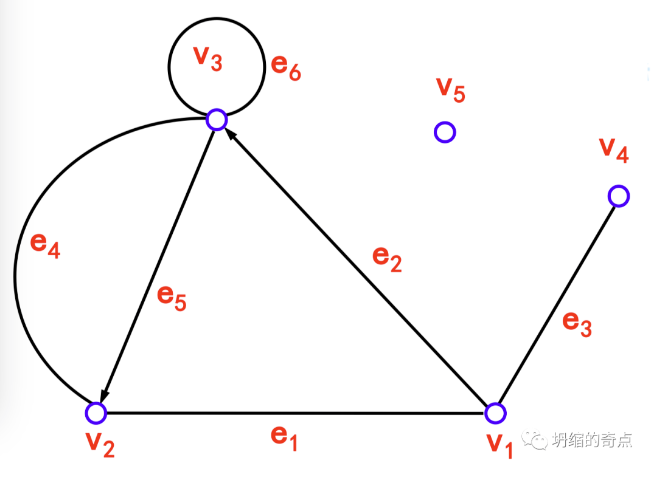
\includegraphics[width=0.5\textwidth]{asset/20231227145030.png}
  \caption{}
  \label{fig:img25_1}
\end{figure}

这道题就是这个样子,有些边是有向的,有些边是无向的. 这个信息区分就是通过是圆括号还是尖括号来区分. 尖括号就表示它是一个有向边,圆括号的就是无向的,也就没有箭头. 这其中,$e_1, e_3, e_4, e_6$是无向边, $e_2, e_5$是有向边. 具体的这些点是要画在什么样的一个位置,其实压根不重要. 

比如V5这个点是一个孤立的点. 它是一个孤点,那你画在任意地方都一样,都可以. 只要不改变这个图的本身结构就行. 你不能V3和V5连上,那这个就不行了. 

接下来,我们来看一道相反的题, 就是我们知道了图形表示, 现在需要我们将其转成集合表示. 我们已知图$G=<V,E>$的图形表示如图\ref{fig:img25_2}, 写出相应的G的集合表示. 

\begin{figure}[ht]
  \centering
  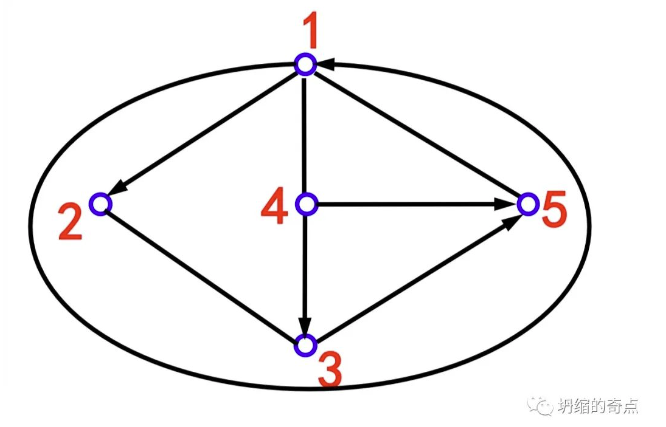
\includegraphics[width=0.5\textwidth]{asset/20231227145043.png}
  \caption{}
  \label{fig:img25_2}
\end{figure}

这个其实也很简单,就是分两步,一个求v一个求e. 首先看一下总共有几个顶点,然后分别把它们写成一个集合. 再之后,这些顶点又有多少个边相互连接,哪些边是有向的,哪些边是无向的. 其答案如下: 

\begin{align*}
  G & = <V, E> \\ & = <\{1, 2, 3, 4, 5\}, \{<1, 1>,<1, 2>,(1, 4),(1, 5),(2, 3),<3, 5>,<4, 3>,<4, 5>\}>
\end{align*}

题目不难,就是一种转换. 带着大家熟悉一下两种表现形式. 大家这时候不要嫌麻烦,或者偷懒. 这个其实很简单,但是很多东西如果不去自己尝试一下,你不会发现一些可能之前发现不了的东西. 不下笔的话往往不会了解到一些信息. 这个只有自己去尝试了之后才能明白. 

一些点需要给大家说一下,就是这些边的表现形式非常多样,外面那个大圈就是由1那一点引出来的,转转转回到了自己本身,这样画是OK的. 如果我们在这里只是画一个小小的圆圈,同样表示这个边,这两个是等价的. 

画成这种形状,这里这个图画成这种形状是否代表着我这个它包含的里面2345的这些点呢? 其实是没有任何关系的. 这个图里不存在什么包含不包含的这种关系,别看它好像给这些围起来了,里面的点好像是被它围在中间一样,不是这个样子的,所以这些边、点的表现形式非常多. 更多的时候我们是看怎么样美观,怎么样写起来画起来比较工整. 

这题答案,集合表现就是$G=<V,E>$,再把$v$和$e$给拆开,$v$是一个集合,所以用花括号表示. 它就是这5个点: $1, \quad 2, \quad 3, \quad 4, \quad 5$, 很简单. 关键是这些边, 我们要把这些边给找出来. 这个边其实你一个一个去找, 按顺序去找就行了. 它有几条边, 它有哪一个指向找出来. 再按照这样的顺序, 把这些点给找出来, 在这个集合里面. 

因为集合本身是一种无序的一种结构, 所以在这里顶点集写成$\{1, \quad 2, \quad 3, \quad 4, \quad 5\}$. 但是如果写成一个非常乱的顺序,比如$\{2, \quad 4, \quad 3, \quad 5, \quad 1\}$也完全可以, 完全等价. 

学习这些不要纠结这些东西,你要知道它是一个无序结构,所以你怎么样写都OK. 为什么我们一般写成这种顺序结构呢? 就是美观,比较符合人类的阅读习惯. 如果你非写成一个乱序, 压根就不算错. 同样对于e里面, e这个集合, 也是一个一个括号写. 它里面就是一些边的集合了,在这里,边的顺序可以任意对调. 

关键还有个什么? 就是大家要把这些有向边、无向边要区分开来. 就是这个表示方法容易出错,容易统一的用这个圆括号去表示了,大家尽量避免这个问题. 

说完了这个两种表现形式之后,我们再来看一下它们各自有什么优缺点. 

首先,集合表示的优点是可以精确描述图的组成信息. 因为我们已经把组成这个图的两个基本要素,一个是顶点,一个是边都给它罗列出来了. 所以它是非常精确的. 集合表示的缺点就是比较抽象,不易于直观理解. 这个是很明显的,尤其是我们说到边,比如说我给你这个集合表现形式,虽然我告诉你哪些点有哪些边,但是你不可能像图这样一眼望过去就知道哪两个点之间有这些边连接,以及这些边是否有向还是无向,有向的话是由哪个点指向哪一个点,这里面有没有环. 都不是那么直接容易看出来的. 

再来看看图形表示,图形表示的优点就是集合表示的缺点反过来了,因为它可以很直观形象地表示出来,所以易于我们人类去理解. 但是它有一个致病的缺点,如果这个图里面的结点或者边数量比较小的话,那用图来表示完全可以,而且非常直观. 但是如果结点以及边数量非常多,几千亿个,就像这个宇宙中的这种类银河系的这种系外星系,或者超星系团,数以千万计或者说数以亿计,如果要用图形表示的话,那就不可能了. 那你得画到什么时候? 计算机即便能画出来,人也看不过来. 

所以说,他们俩各自都有一些优缺点. 

那我们关于图的表示只有这两种方式了吗? 一个图形表示,一个集合表示. 其实并不是,其实图的表示是一个三国争霸的状态, 还有一霸没有出现, 这个一霸就叫做矩阵表示. 

在这里将它列出来给大家看一下: 

\begin{align*}
  A_G = \begin{bmatrix}
  0 & 1 & 0 & 0 & 1 & 1 \\  
  1 & 0 & 1 & 0 & 0 & 0 \\
  0 & 1 & 1 & 1 & 0 & 1 \\ 
  0 & 0 & 1 & 0 & 1 & 1 \\ 
  1 & 0 & 0 & 1 & 0 & 1 \\
  1 & 0 & 1 & 1 & 1 & 0
  \end{bmatrix} 
\end{align*}

这里列出来的这种形式就是矩阵表示. 是不是很疑惑,这个矩阵表示是怎么样去表示一个图的呢? 

除了集合以及图形表示之外,为什么会多出来这么一种矩阵表示? 因为我们很多时候,尤其是进入信息化时代,大部分的数据处理都是用计算机去做的,图也不例外. 我们也希望计算机能帮助我们去处理关于图的这些数据,然而对于计算机而言,集合的形式或者图形的形式都不太适合. 集合的形式输入给电脑里面,电脑它往往也不大明白这个该怎么处理,图形的形式可能更差. 

我们知道,现在人工智能就有一个领域叫做计算机视觉,就是专门让计算机去像人类一样拥有视觉识别的功能. 不过用于处理图可能还是有点勉强. 可是矩阵是一个非常适合计算机的形式,我们上线性代数的时候就知道,在计算机里面我们可以去做矩阵运算,所以就想到用矩阵能不能去表现这些图. 

\section{邻接矩阵}

如果我们用矩阵来表示的话,那我们得先约定一些东西. 本身矩阵和图是两个差别很大,或者说隔得有点远的东西. 那我们怎么样去给它做出一些约束呢? 

\begin{itemize}
  \item 首先,我们这个矩阵里面的这些行列需要有固定的次序,行列的位置不同,代表不同的矩阵
  \item 其次,需要讲图中的结点按某种既定顺序排列
  \item 再次,若并未给出具体排序,则顺序默认为书写结点集V时的结点顺序. 
\end{itemize}

我们知道,即便仅仅是行列的位置不同这两个矩阵也是完全不同的. 比如我把这个2*2的矩阵第一行1、2,第二行3、4做一下转置,那第一行就变成1,3,第二行就变成2、4. 这就表示成两个不同的矩阵了. 

所以矩阵的行列是有一个固定的次序的,它不能任意的变动. 为了满足这个条件,我们需要需要将图中的结点按照某种既定的顺序做个排列. 如果你没有按照这种规则去做出排列,那我们这种顺序就默认成书写这个结点集V的时候的结点顺序. 

比如我们有5个点,就像我们之前那道题里面\{1,2,3,4,5\},分别标号是$1,2,3,4,5$, 是5个点. 如果写成$\{3,5,2,1,4\}$, 没有给它一个具体的排序方式的话, 我们就可以按照$3,5,2,1,4$这种顺序去约定它. 第一个点就对应着标号为3这个点,第二个点就是标号为5的这个点,以此类推,$3,5,2,1,4$. 

好,说到这里可能大家还不是很明白为什么要做这种约束. 接下来就需要用到刚才说的一个内容了,设这个图是$G=<V,E>$, 其中$V=\{v1,v2,...,vn\}$, 并且已经确定了各结点的排列次序, 则将n阶方阵$A_G=(a_{ij})_{nxn}$称为$G$的邻接矩阵,其中: 

\begin{align*}
a_{ij}=\begin{cases}1, \mbox{若}V_i\mbox{与}V_j\mbox{间有边} \\ 0, \mbox{若}V_i\mbox{与}V_j\mbox{间无边} \end{cases}
& i,j = 1, 2, ..., n
\end{align*}

这个邻接矩阵里面的每一个元素$a_{ij}$它代表了代表了这个矩阵里面第i行、第j列的这个元素. 它的取值只有1和0. 这个逻辑关系其实非常简单,就是说你vi这个点和vj这个点如果是有边连接的话,你对应的这个元素就是1,如果两个点之间没有边的话,那它就是0,这个是只有两个取值的. 所以这个邻接矩阵本身的取值是非常简单. 取1还是取0就完全取决于e,就是看e. 如果有边就是1,无边就是0. 

我们接下来看一个例子,给出了一个图$G$ \ref{fig:img25_3}, 写出图$G$的邻接矩阵. 

\begin{figure}[ht]
  \centering
  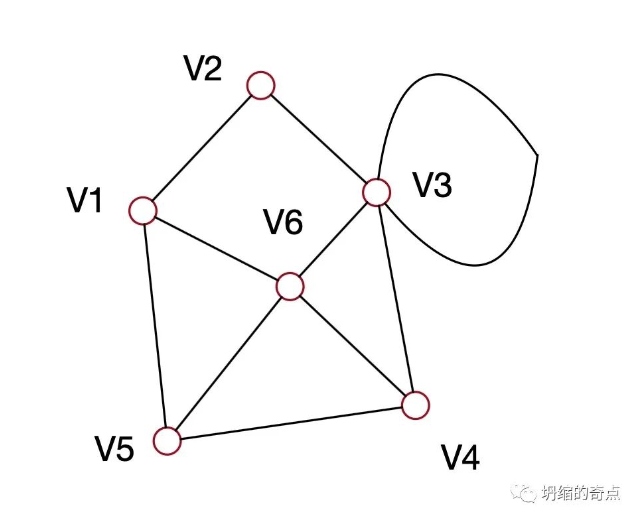
\includegraphics[width=0.4\textwidth]{asset/20231227145100.png}
  \caption{}
  \label{fig:img25_3}
\end{figure}

这个里面总共有V1到V6总共有6个点,我们就按照这个下标的顺序来给它做个排列. 

按照下标的顺序排列也就是说行方向是按照V1到V6的方向,列方向也是按照V1到V6的这个方向去排布. 然后我们会观察到,行和列所交的位置代表了V1和V2之间有没有连线. 如果有的话就是1,没有的话就是0. 

大家可以去自己尝试一下,你就看一下矩阵列出来是怎样一个形式. 我这里给大家列一下, 如图\ref{fig:img25_4}: 

\begin{figure}[ht]
  \centering
  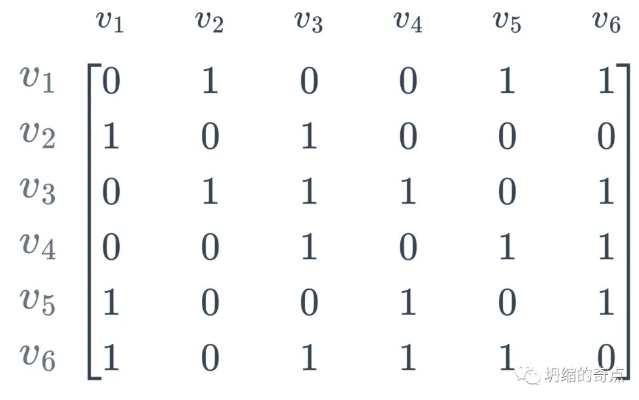
\includegraphics[width=0.6\textwidth]{asset/20231227145115.png}
  \caption{}
  \label{fig:img25_4}
\end{figure}

因为V1、V6都是一样的,大家会发现这个矩阵其实是一个对称的结构. 因为, 行1列2是表示V1和V2连线,是1,行2列1呢,同样表示V1和V2的连线,也是1. 所以对于无向图而言,邻接矩阵就是一个对称的结构,是一个沿对角线对称的结构. 

但是如果是一个有向图的话那就不一样了,这个时候约定V1行代表了由V1指向的点,如果在这里V1、V2之间的这条边是由V1指向V2的,方向是指向V2的,在行1,它代表V1指向V2. 但是如果在行2就又不一样了,代表了由V2指向V1. 

我们再反过来看,如果箭头是由V1指向V2的话,并没有一条边由V2指向V1,在这里它就是0了. 所以有向图无向图在这方面会稍微有点不一样,大家注意一下就OK了,其实它表达的意思呢很简单. 

\begin{align*}
  A_G = \begin{bmatrix} 
  0 & 1 & 0 & 0 & 1 & 1 \\  
  1 & 0 & 1 & 0 & 0 & 0 \\
  0 & 1 & 1 & 1 & 0 & 1 \\ 
  0 & 0 & 1 & 0 & 1 & 1 \\ 
  1 & 0 & 0 & 1 & 0 & 1 \\
  1 & 0 & 1 & 1 & 1 & 0
  \end{bmatrix}
\end{align*}

写成这个形式的就跟刚才一样了. 

那么我们刚才呢说了很多这种约束条件,就比如说这个图的邻接矩阵,因为行和列位置交换一下的话都对应着不同的矩阵,所以我们说了要约定这个节点或者说顶点的一个默认排序. 那在这里我们探讨一下,图的这个邻接矩阵这个矩阵的形式是唯一的吗? 

\begin{itemize}
  \item 一般而言,同一个图按照不同的顶点排列次序,写出的邻接矩阵形式上是不同的,但是相互之间可以通过调换某些行或列的位置而得到. 
  \item 对邻接矩阵的行或列进行交换,对应的实际上是在对顶点的排序中调换顶点的位置. 
  \item 若不考虑顶点排序的不同产生的邻接矩阵的不同,则图与邻接矩阵之间是一一对应的. 
  \item 实际操作上,往往略去顶点排序不同导致的邻接矩阵的多样性, 选择任意一种顶点次序得出的邻接矩阵作为该图的邻接矩阵. 
\end{itemize}

以上几句话的意思就是告诉大家,不要纠结,你选定一个之后,把这个顶点的排列顺序给写下来,然后我们就按照这个顺序去做这个邻接矩阵就行了. 不用去管它有可能会有其他形式的一个排列,其他形式的排列你不能说它不合理,都是合理的,但是不用去管那些. 就按照你写的这个去做就可以了. 

在说了图的邻接矩阵之后,我们已经学了三种图的表现形式了. 一个集合表示、一个图形表示、还有矩阵的一个表现形式. 接下来,我们要来看看图的种类. 

\section{图的种类}

其实图的分类方法也有非常多种,首先按照它这个边有没有方向我们可以分成3类. 一类是有向的, 如图\ref{fig:img25_5}, 一类是无向图, 就是它这个边都没有方向的, 如图:\ref{fig:img25_6}: 

\begin{figure}[ht]
  \centering
  \begin{minipage}[h]{0.4\textwidth}
    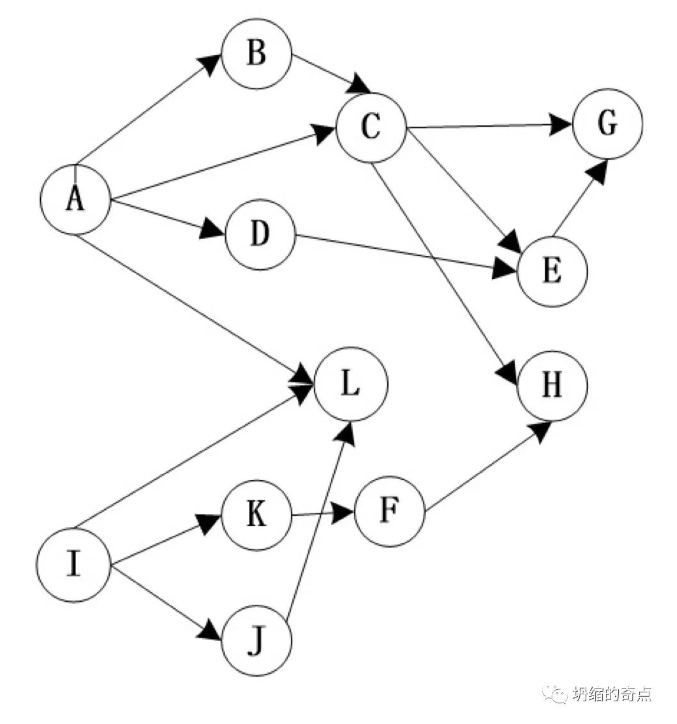
\includegraphics[width=\textwidth]{asset/20231227145133.png}
    \caption{}
    \label{fig:img25_5}
  \end{minipage}%
  \hspace{1em}
  \begin{minipage}[h]{0.4\textwidth}
    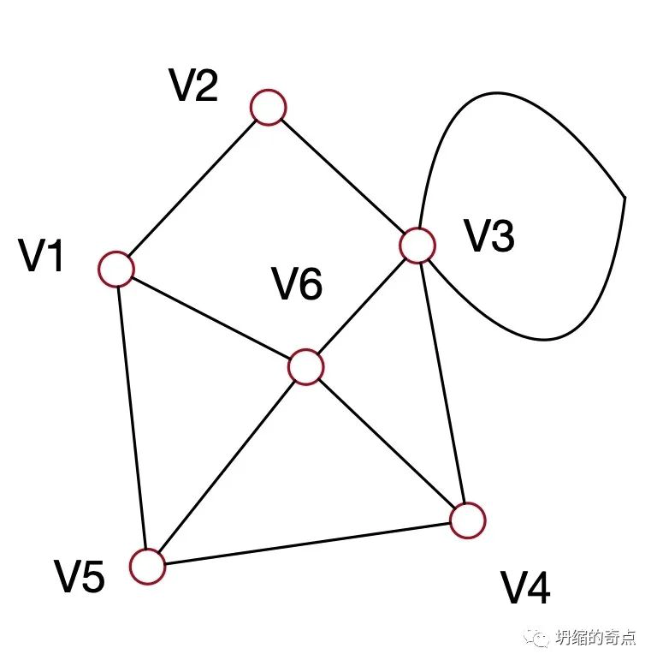
\includegraphics[width=\textwidth]{asset/20231227145141.png}
    \caption{}
    \label{fig:img25_6}
  \end{minipage}
\end{figure}

还有一类就是混合图, 如图\ref{fig:img25_7}, 混合图就是里面既有有向的边, 也有无向的边, 这种叫做混合图. 

\begin{figure}[ht]
  \centering
  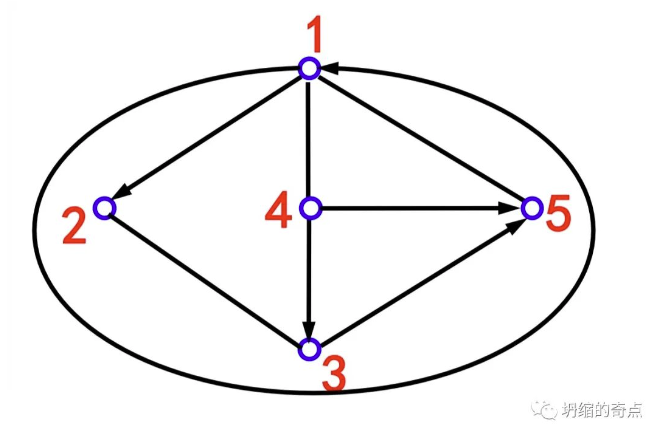
\includegraphics[width=0.5\textwidth]{asset/20231227145154.png}
  \caption{}
  \label{fig:img25_7}
\end{figure}

混合图大家不要觉得奇怪,往往也会有一些实际运用. 它这些边看似感觉像是没有方向的,但是实际上它代表了一对方向相反的连接相同端点的一对. 在混合图中,可以将无向边转换为方向相反的两条有向边来处理, 如图\ref{fig:img25_8}: 

\begin{figure}[ht]
  \centering
  \begin{minipage}[h]{0.4\textwidth}
    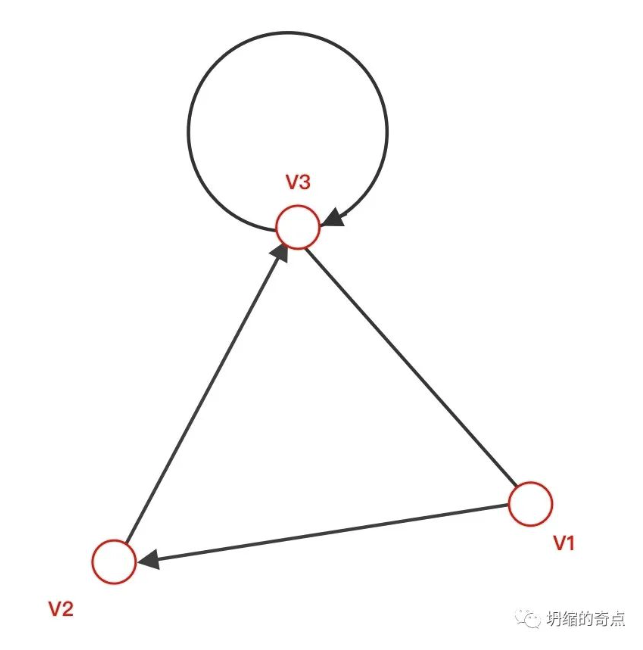
\includegraphics[width=\textwidth]{asset/20231227145210.png}
  \end{minipage}%
  \hspace{1em}
  \begin{minipage}[h]{0.4\textwidth}
      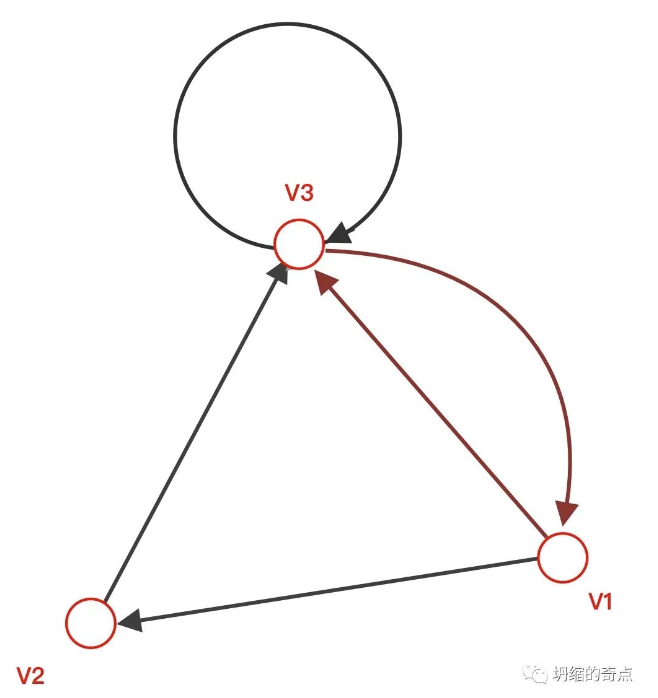
\includegraphics[width=\textwidth]{asset/20231227145222.png}
  \end{minipage}
  \caption{}
  \label{fig:img25_8}
\end{figure}

为什么要做这样的转换呢? 因为我们知道有向边和无向边的处理是有点不一样,就像我们在写程序的时候,把一个int和一个浮点型的变量加在一起的话,这个程序自动的会做一个强制类型转换. 就变成一个精度更高的浮点型的形式. 

如果按照图的里面有无平行边(重边)来分类的话,可以分成以下几类(图:\ref{fig:img25_9}, \ref{fig:img25_10}, \ref{fig:img25_11}): 

\begin{figure}[ht]
  \centering
  \begin{minipage}[t]{0.3\textwidth}
    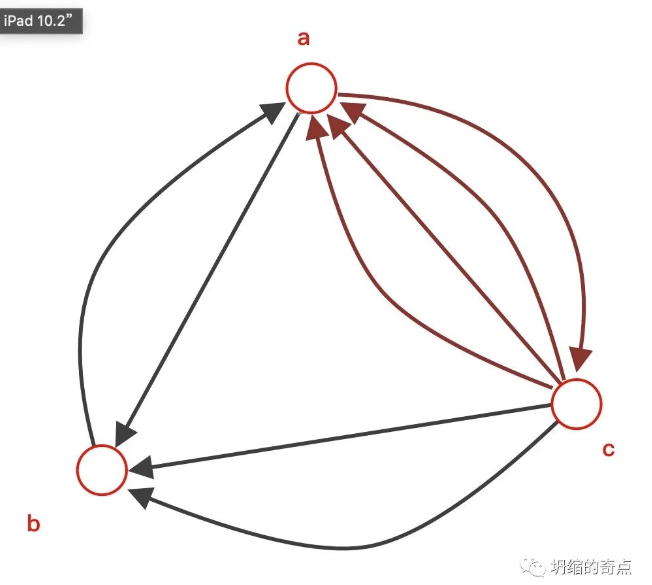
\includegraphics[width=\textwidth]{asset/20231227145235.png}
    \caption{多重图: 有平行边的图}
    \label{fig:img25_9}
  \end{minipage}%
  \hspace{0.5em}
  \begin{minipage}[t]{0.3\textwidth}
    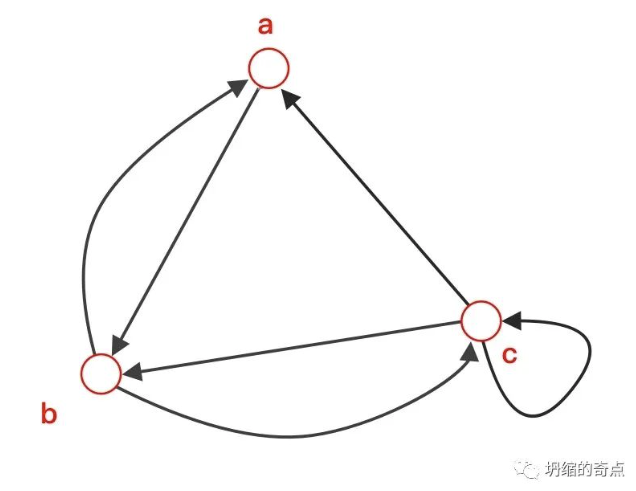
\includegraphics[width=\textwidth]{asset/20231227145249.png}
    \caption{线图: 无平行边的图}
    \label{fig:img25_10}
  \end{minipage}%
  \hspace{0.5em}
  \begin{minipage}[t]{0.3\textwidth}
    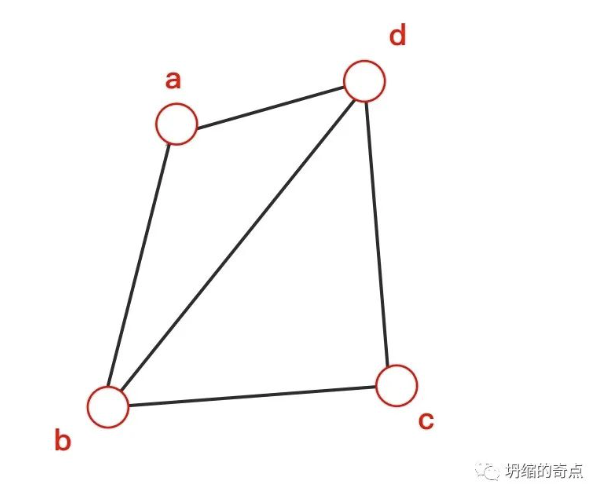
\includegraphics[width=\textwidth]{asset/20231227145259.png}
    \caption{简单图: 无环的线图}
    \label{fig:img25_11}
  \end{minipage}
\end{figure}

简单图和线图之间的区别, 就是看它有没有环. 

还有一种分类方法,按边,或者顶点是否赋于权重进行分类,氛围赋权图和无权图. 

赋权图: G是一个三重组$<V,E,g>$或四重组$<V,E,f,g>$, 其中V是结点集合,E是边的集合,f是V到负实数集合的函数,g是从E到非负实数集合的函数. 

关于「权」,我们刚才所说的,包括之前那个高铁线路的例子里面,高铁线路里面线段的长度并不代表真实的这个线段长度的关系. 图边的长度并不能代表任何东西,没有任何含义. 当然在这我们就可以通过赋予权重的形式来给图更多的实际意义. 

赋权图其实和图的定义非常相似,只不过就是多了一个或者两个函数. f是关于V,也就是从顶点到非负实数的一个映射函数. 它可以把每一个顶点赋予一个非负实数. g是给每一条边赋予一个非负实数,它们都是一个函数. 

\begin{figure}[ht]
  \centering
  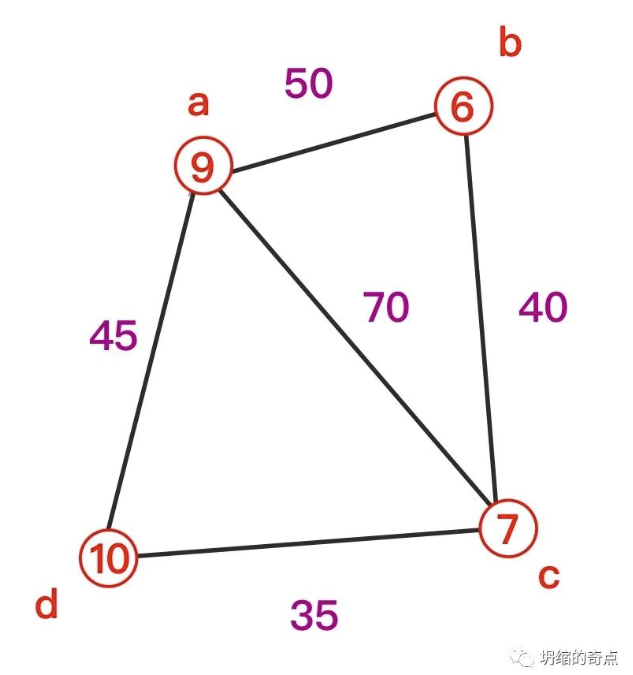
\includegraphics[width=0.5\textwidth]{asset/20231227145314.png}
  \caption{}
  \label{fig:img25_12}
\end{figure}

图 \ref{fig:img25_12} 中,有a b c d四个点. 现在我们不单单的是只有点和边,给每个顶点赋予了一些数字,同样的给每条边赋予了一些数字. 先不管它这个实际意义是什么,只是一种抽象的数据结构. 我们可以人为的给它这些数字,赋予一些意义. 比如说可以表示距离,a、d和b、d之间的一个距离. 

顶点的数值又代表了城市的半径有多大,我们可以根据自己的需要去赋予它实际意义. 但是它对应的这种数据的数学抽象模型都是一样的. 

我们根据题目里面给的这些数字能不能写出这个相应的函数呢? 

\begin{align*}
  & f_2(a)=9, f_2(b)=6, f_2(c)=7, f_2(d)=10, \\ 
  & g_2((a,b))=50, g_2((a,c))=70, \\ 
  & g_2((a,d))=45, g_2((b,d))=40, g_2((c,d))=35
\end{align*}

其实形式也非常简单,我们就需要注意一下关于顶点一般约定俗称是用f来表示,g是代表了边的函数. 所以在这里,a、b是用这个括号括起来,代表一个边,所以它是套两层括号. 

就是把这个函数名称写出来,然后括号再加上你对应的顶点或者对应的边,数值是多少,就是这么简单. 这个就是赋权图里面函数的写法. 

赋权图函数,这些数字的含义往往在我们一些优化方式里面,尤其是在一些路径规划里面是非常有用的. 有的同学可能是学过像greedy这种弹性算法,它这里面往往针对的就是有这种权重的图去研究的. 因为它要算最短路径,图如果没有赋予它相应的权重的话,那它没有意义. 

还有一件事大家可以注意一下,就是赋权图要么是一个三重组合,要么是一个四重组合. 也就是说,要么是$<V,E,g>$, 要么是$<V,E,f,g>$. 这里面不管是三重还是四重,都包含了g. 而f往往是可有可无的. 

这代表往往大部分情况,如果研究有权图边的权重绝大部分情况下都是有的. 几乎你不会遇到只有顶点有权重而边没有权重这种情况. 顶点可以没有权重,但一般按照实际问题来讨论的话,往往边的权重是会有的. 

现在我们一共了解了三种分类方法,不过大家不要觉得这三种方法是彼此孤立的、只是一个单纯的并列关系,并不是这个样. 往往是综合应用的,比如刚才我们举例的赋权图,全称应该是「无向赋权简单图」. 

首先,它是一个无线的,第二它有权重,第三呢,它是一个简单图,因为它是一个无环的线图. 